\subsection{شبیه‌سازی کانال رول-پیچ استند در حضور کنترل‌کننده LQIDG}
در بخش
\ref{quadchanell_roll_pitch}
شبیه‌سازی کانال رول استند چهارپره انجام شد. در این بخش به بررسی عملکرد چهارپره در حضور کنترل‌کننده LQIDG پرداخته می‌شود. کنترل‌کننده LQDG در بخش‌های
\ref{openloop_game}
و
\ref{closedloop_game}
بررسی شده است.
 در شبیه‌سازی برای بهینه‌سازی ضرایب وزنی از روش
TCACS \cite{Karimi2010}
استفاده شده است.
\begin{figure}[H]
	\centering
	\begin{subfigure}
		\centering
		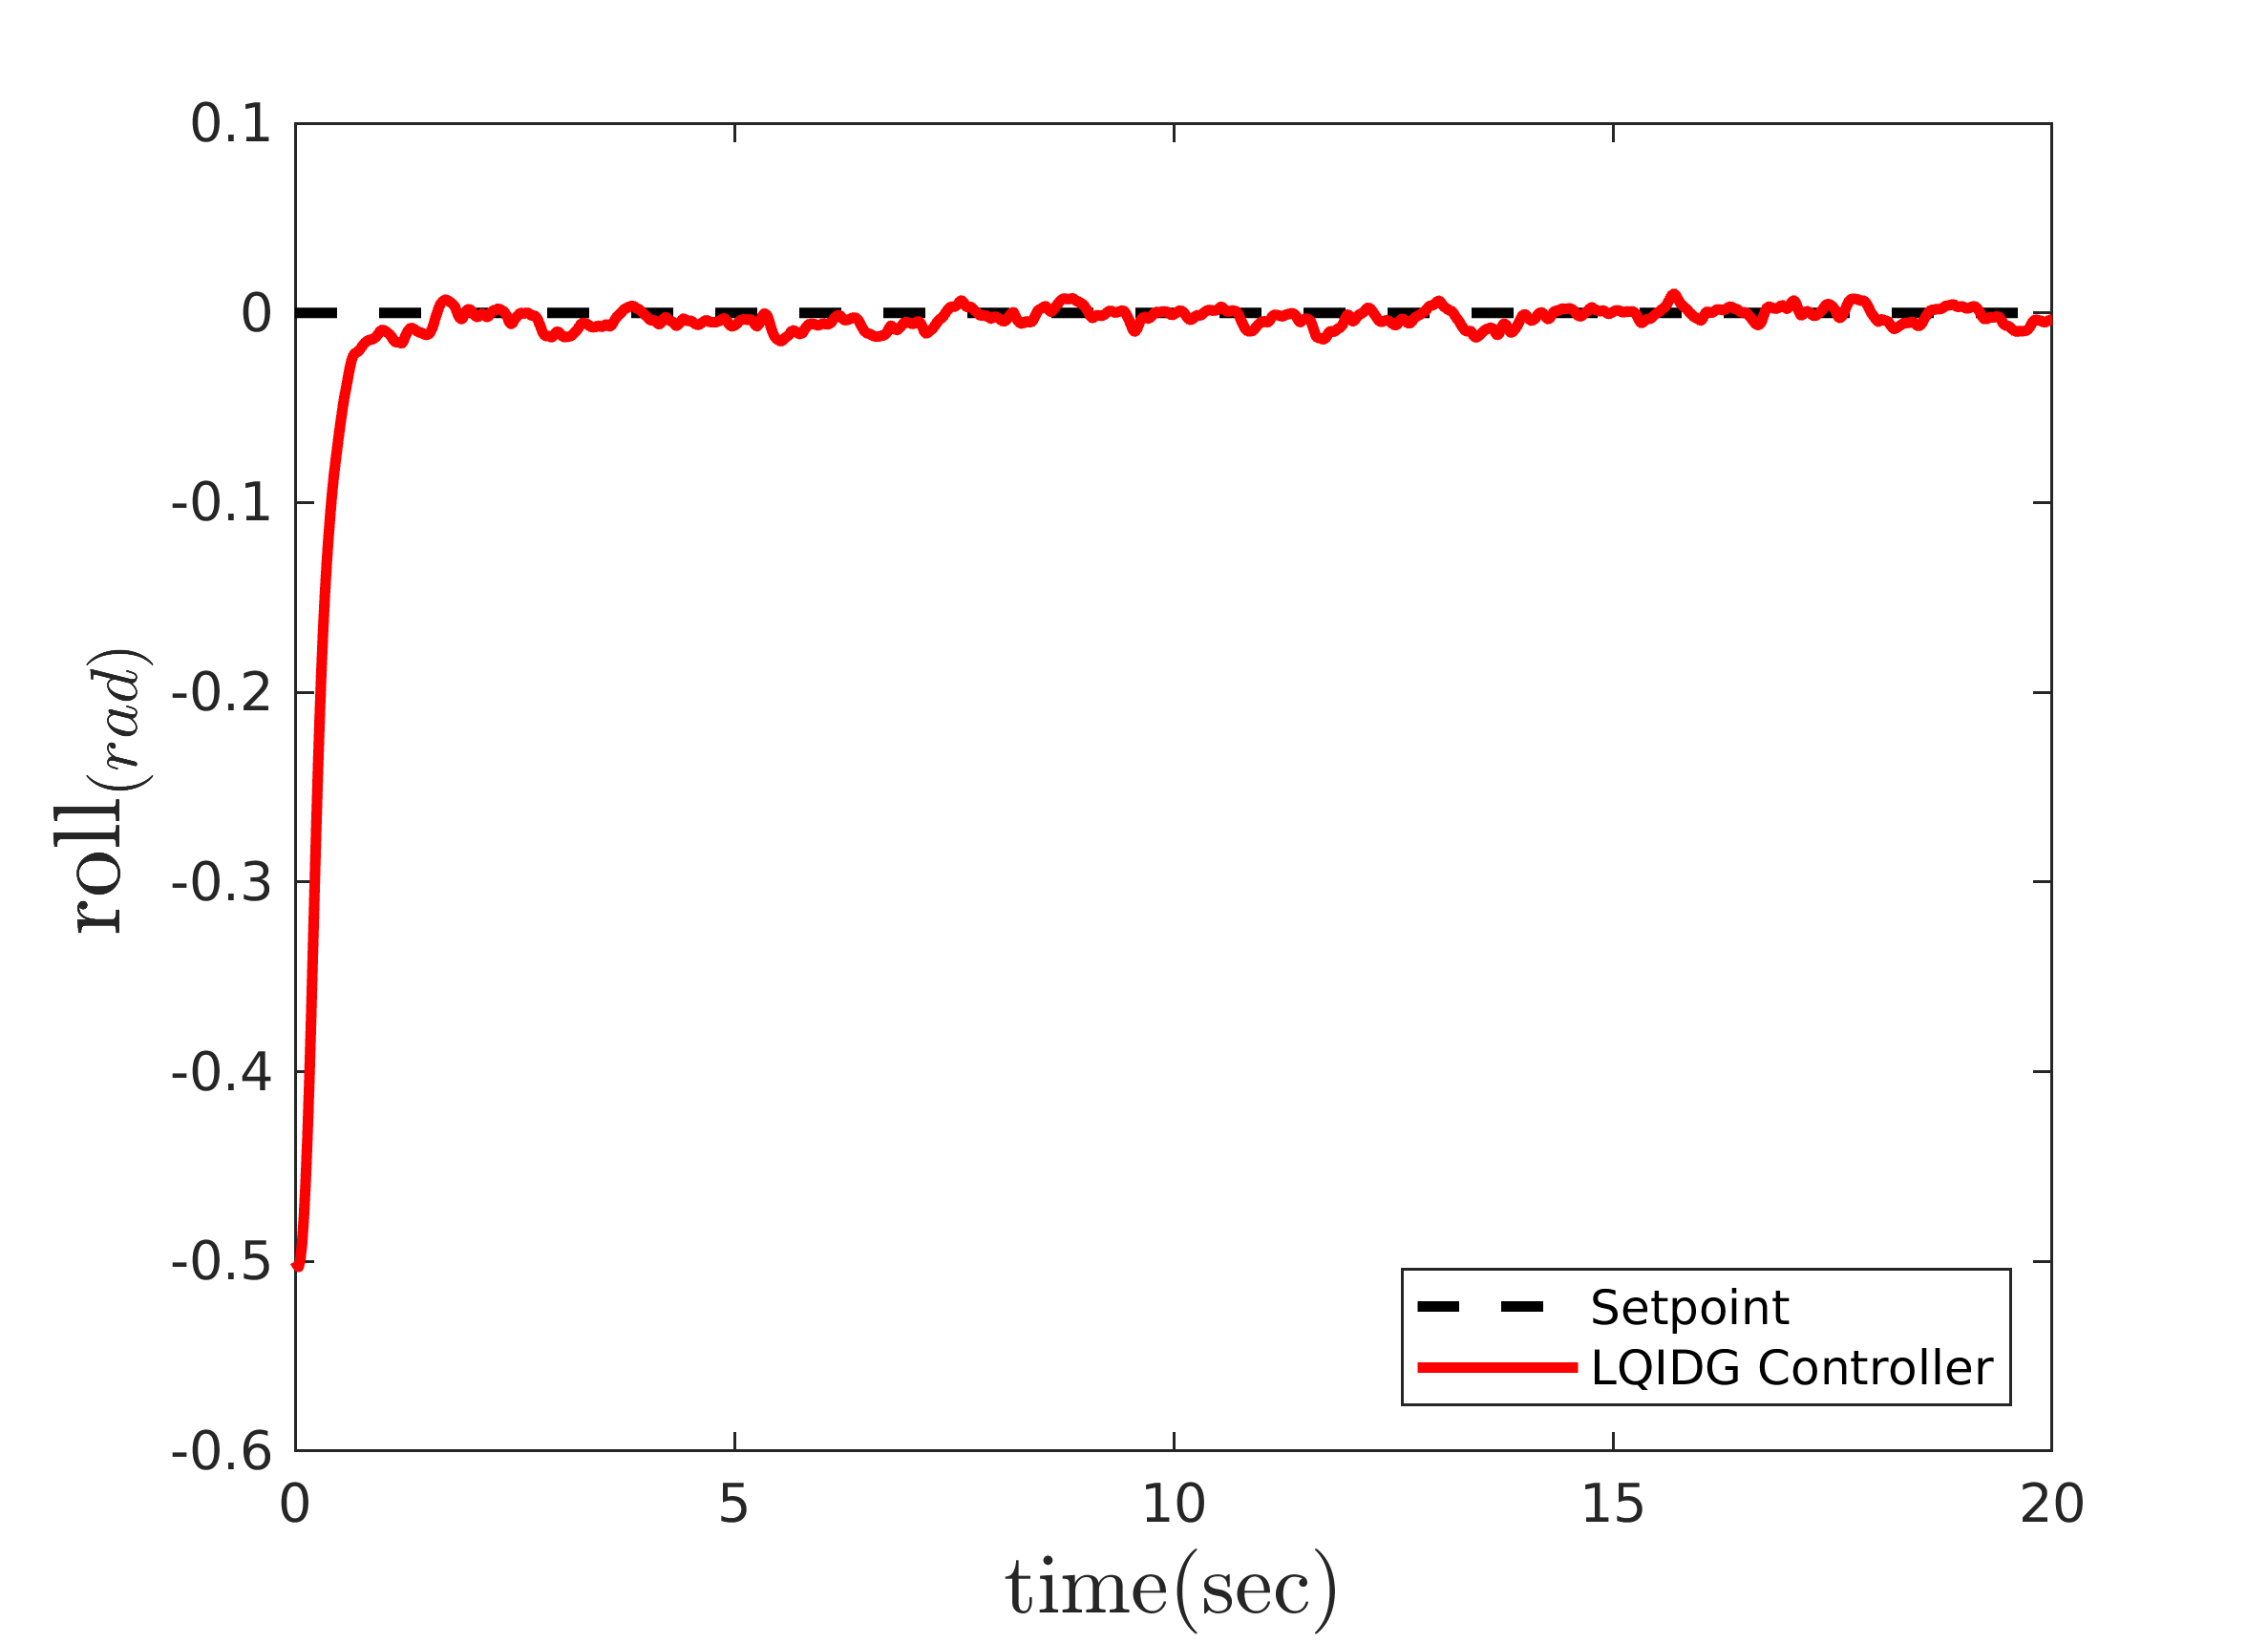
\includegraphics[width=12cm]{../Figures/MIL/LQIDG/Roll_Pitch/lqidg_roll.png}
		\caption{تغییرات زاویه رول}
	\end{subfigure}%
	\begin{subfigure}
		\centering
		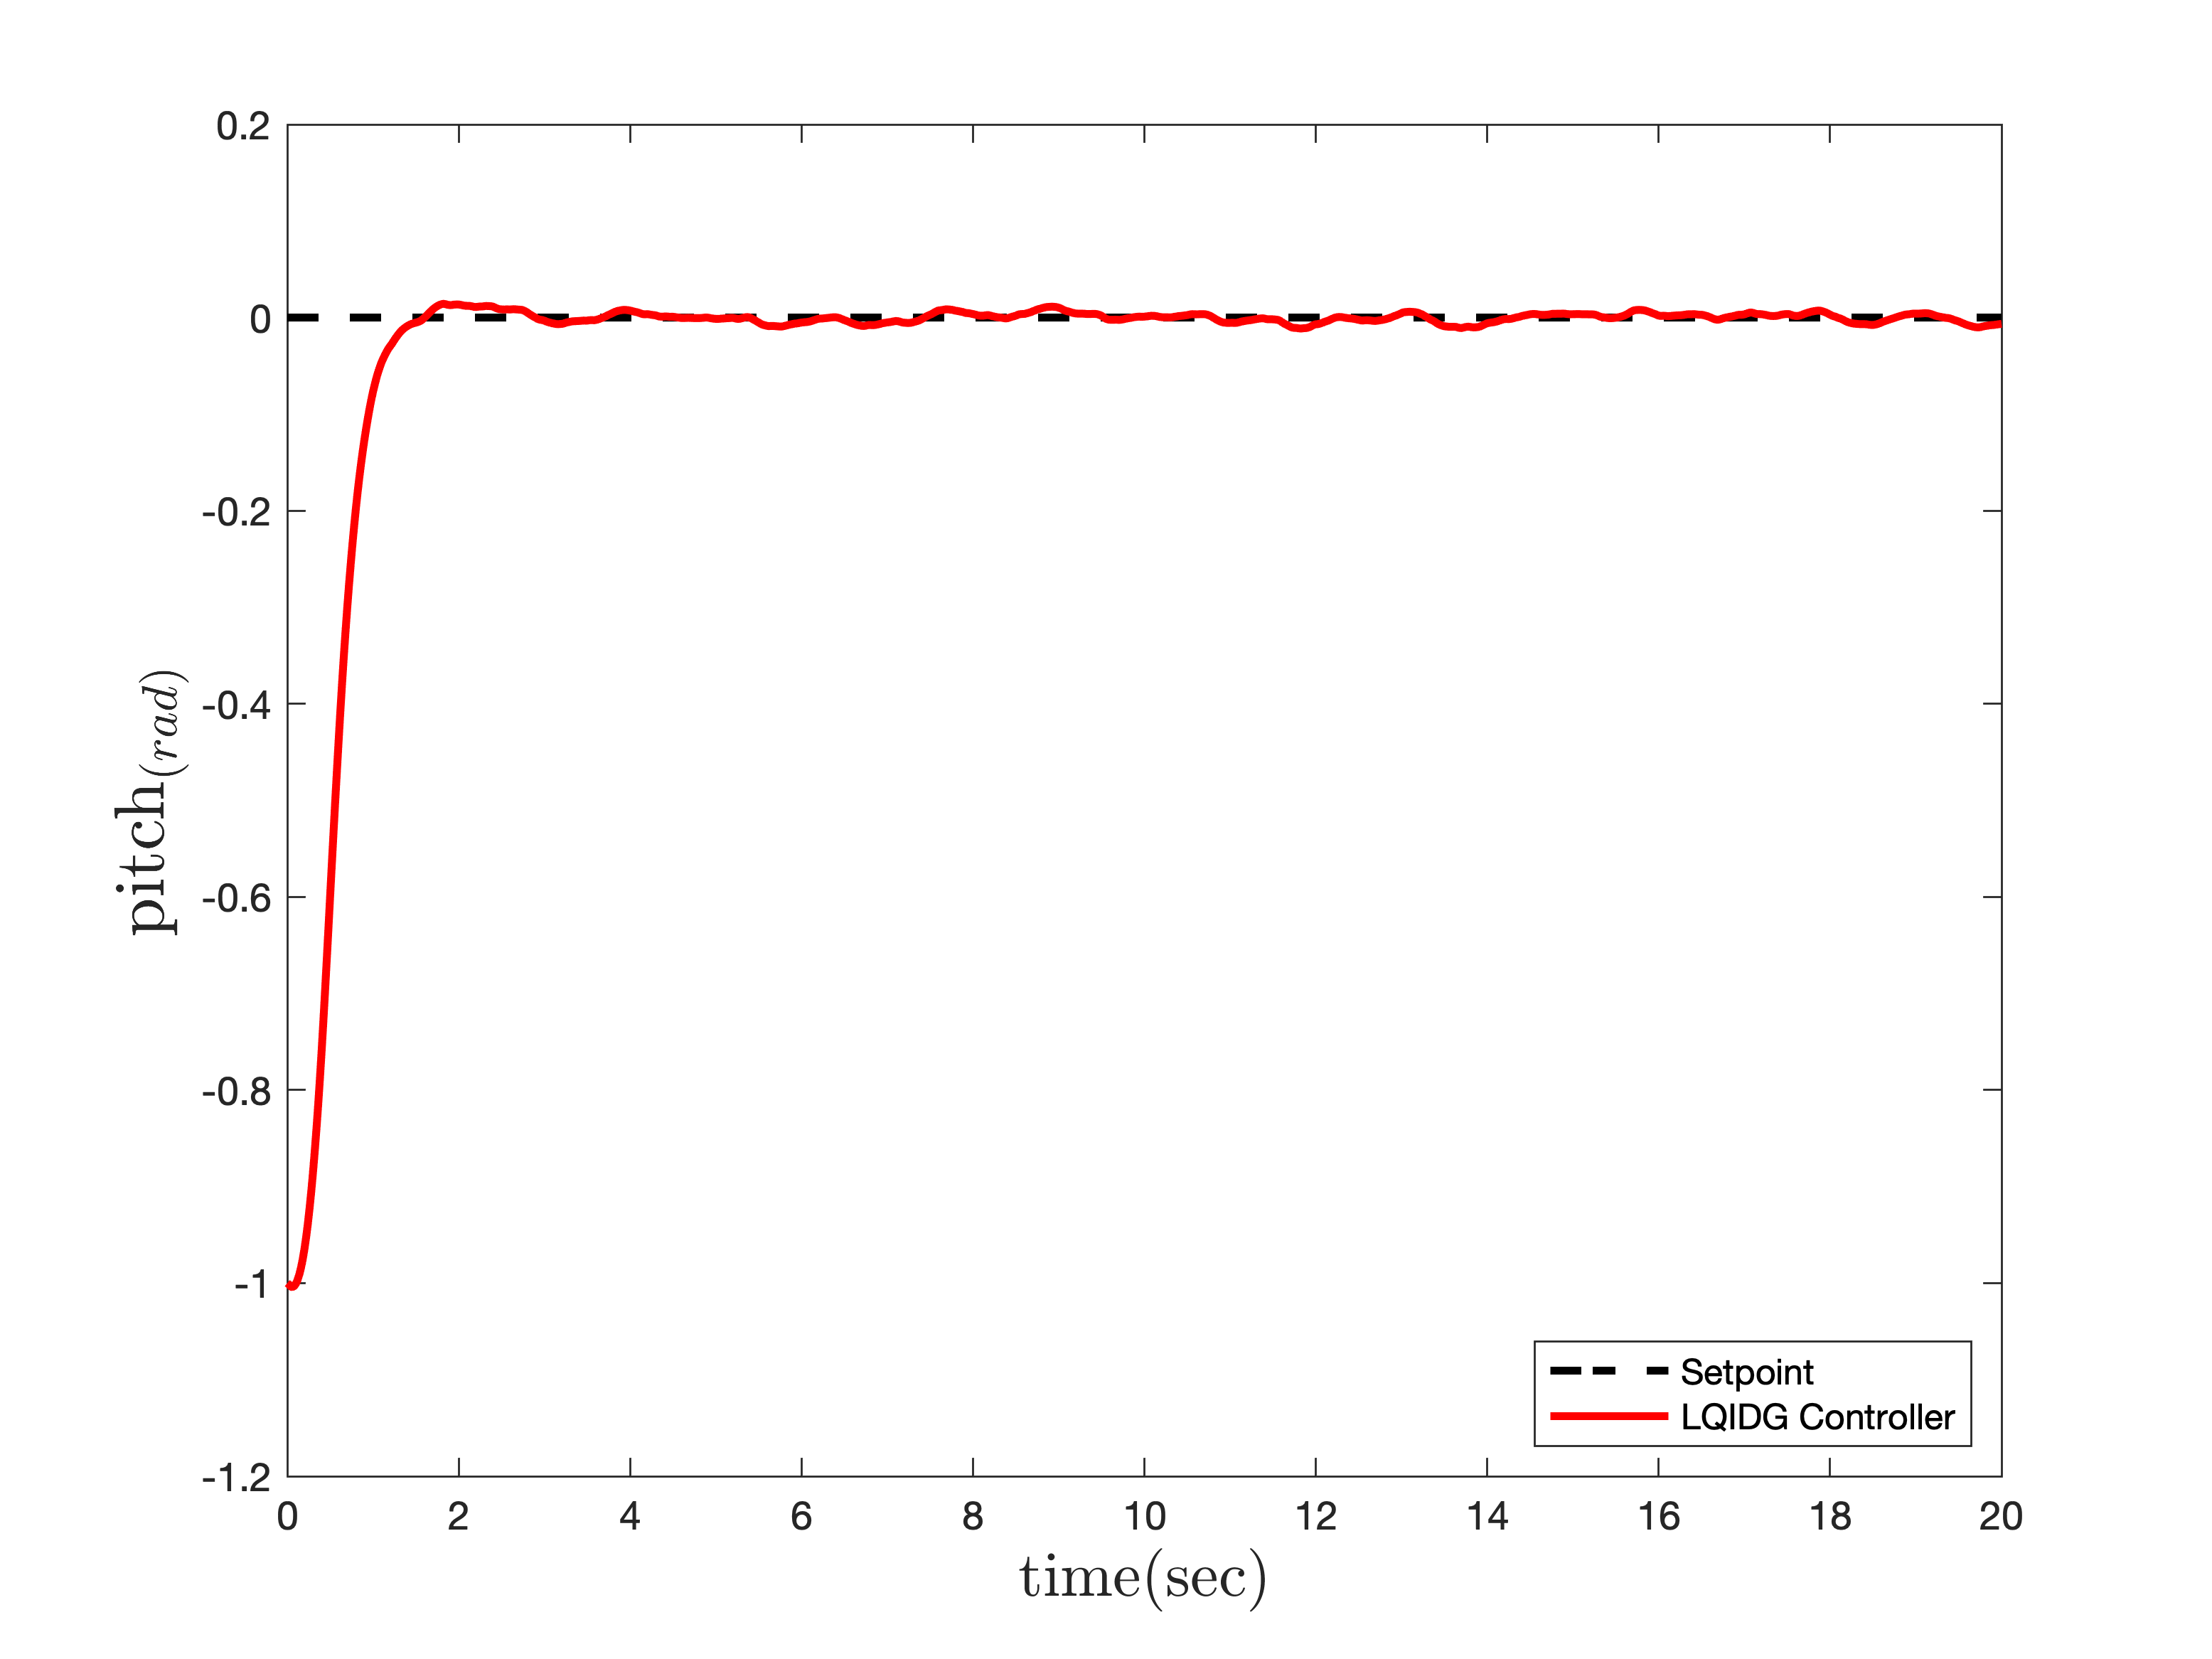
\includegraphics[width=12cm]{../Figures/MIL/LQIDG/Roll_Pitch/lqidg_pitch.png}
		\caption{تغییرات زاویه پیچ}
	\end{subfigure}
	\caption{‫‪عملکرد کنترل‌کننده LQIDG در کنترل زاویه رول و پیچ (تعقیب ورودی صفر)}
\end{figure}


\begin{figure}[H]
	\centering
	\begin{subfigure}
		\centering
		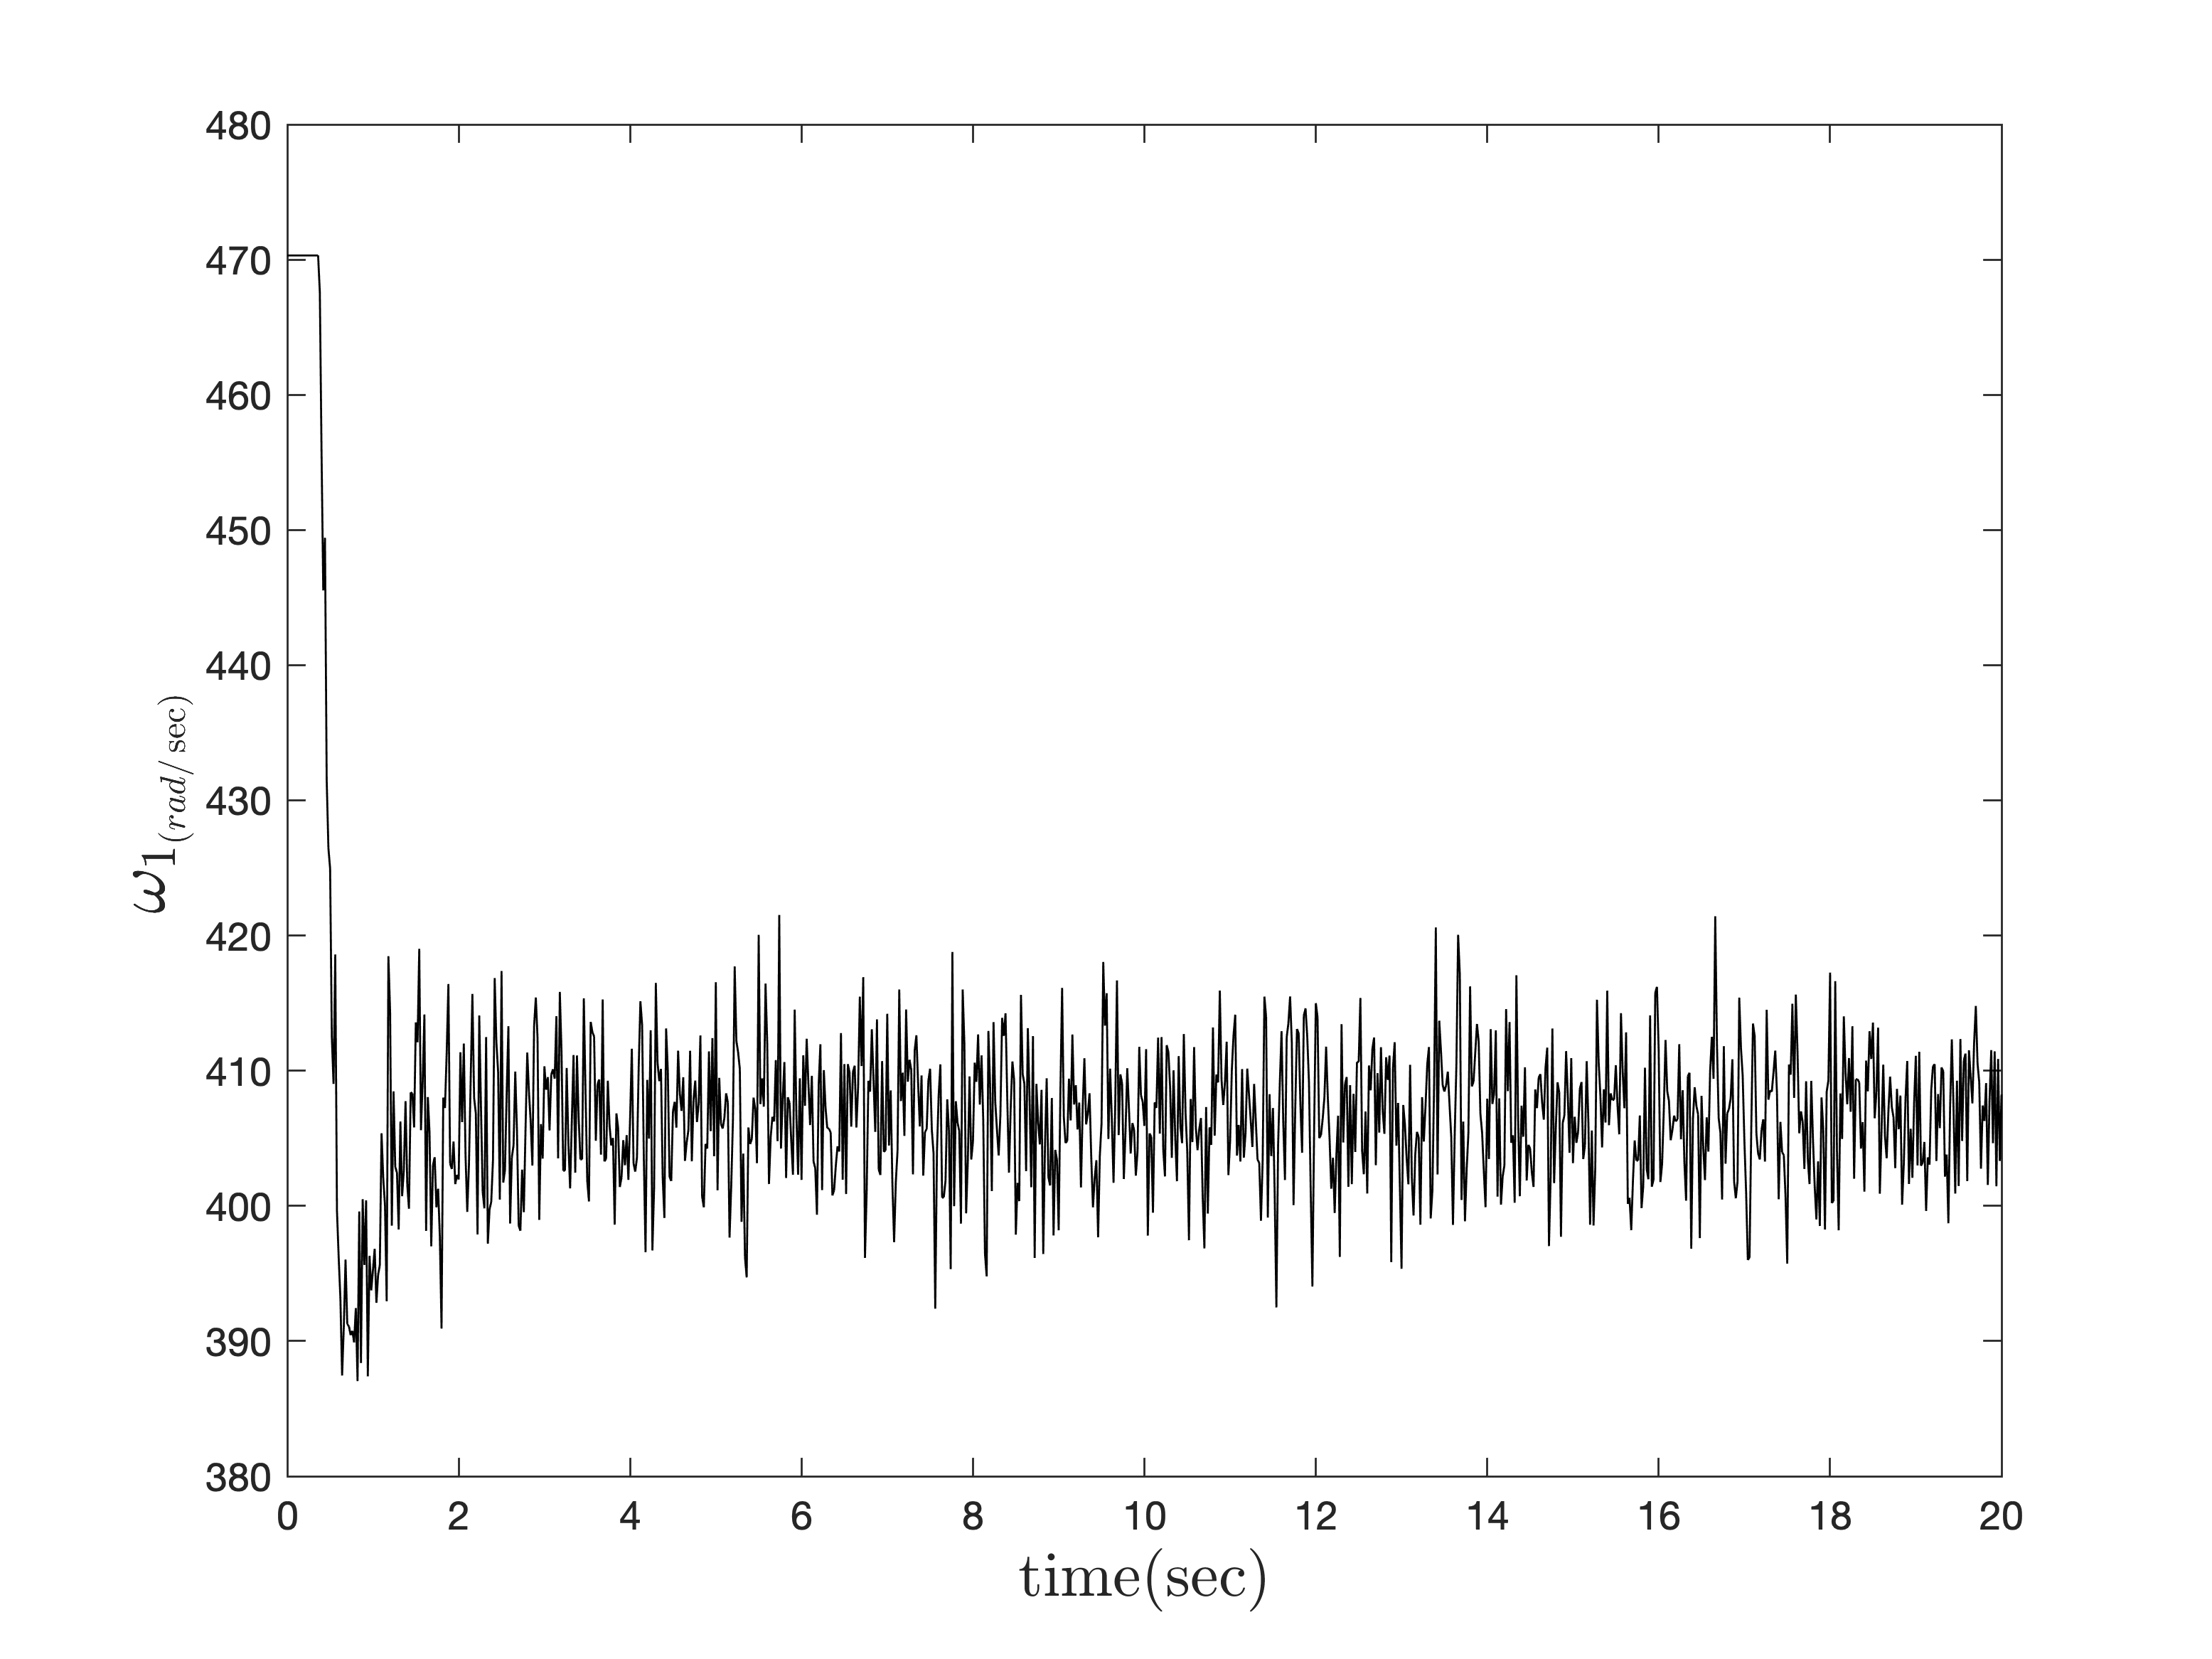
\includegraphics[width=12cm]{../Figures/MIL/LQIDG/Roll_Pitch/lqidg_roll_pitch_Omega_1.png}
		\caption{موتور شماره یک}
	\end{subfigure}
	\begin{subfigure}
	\centering
	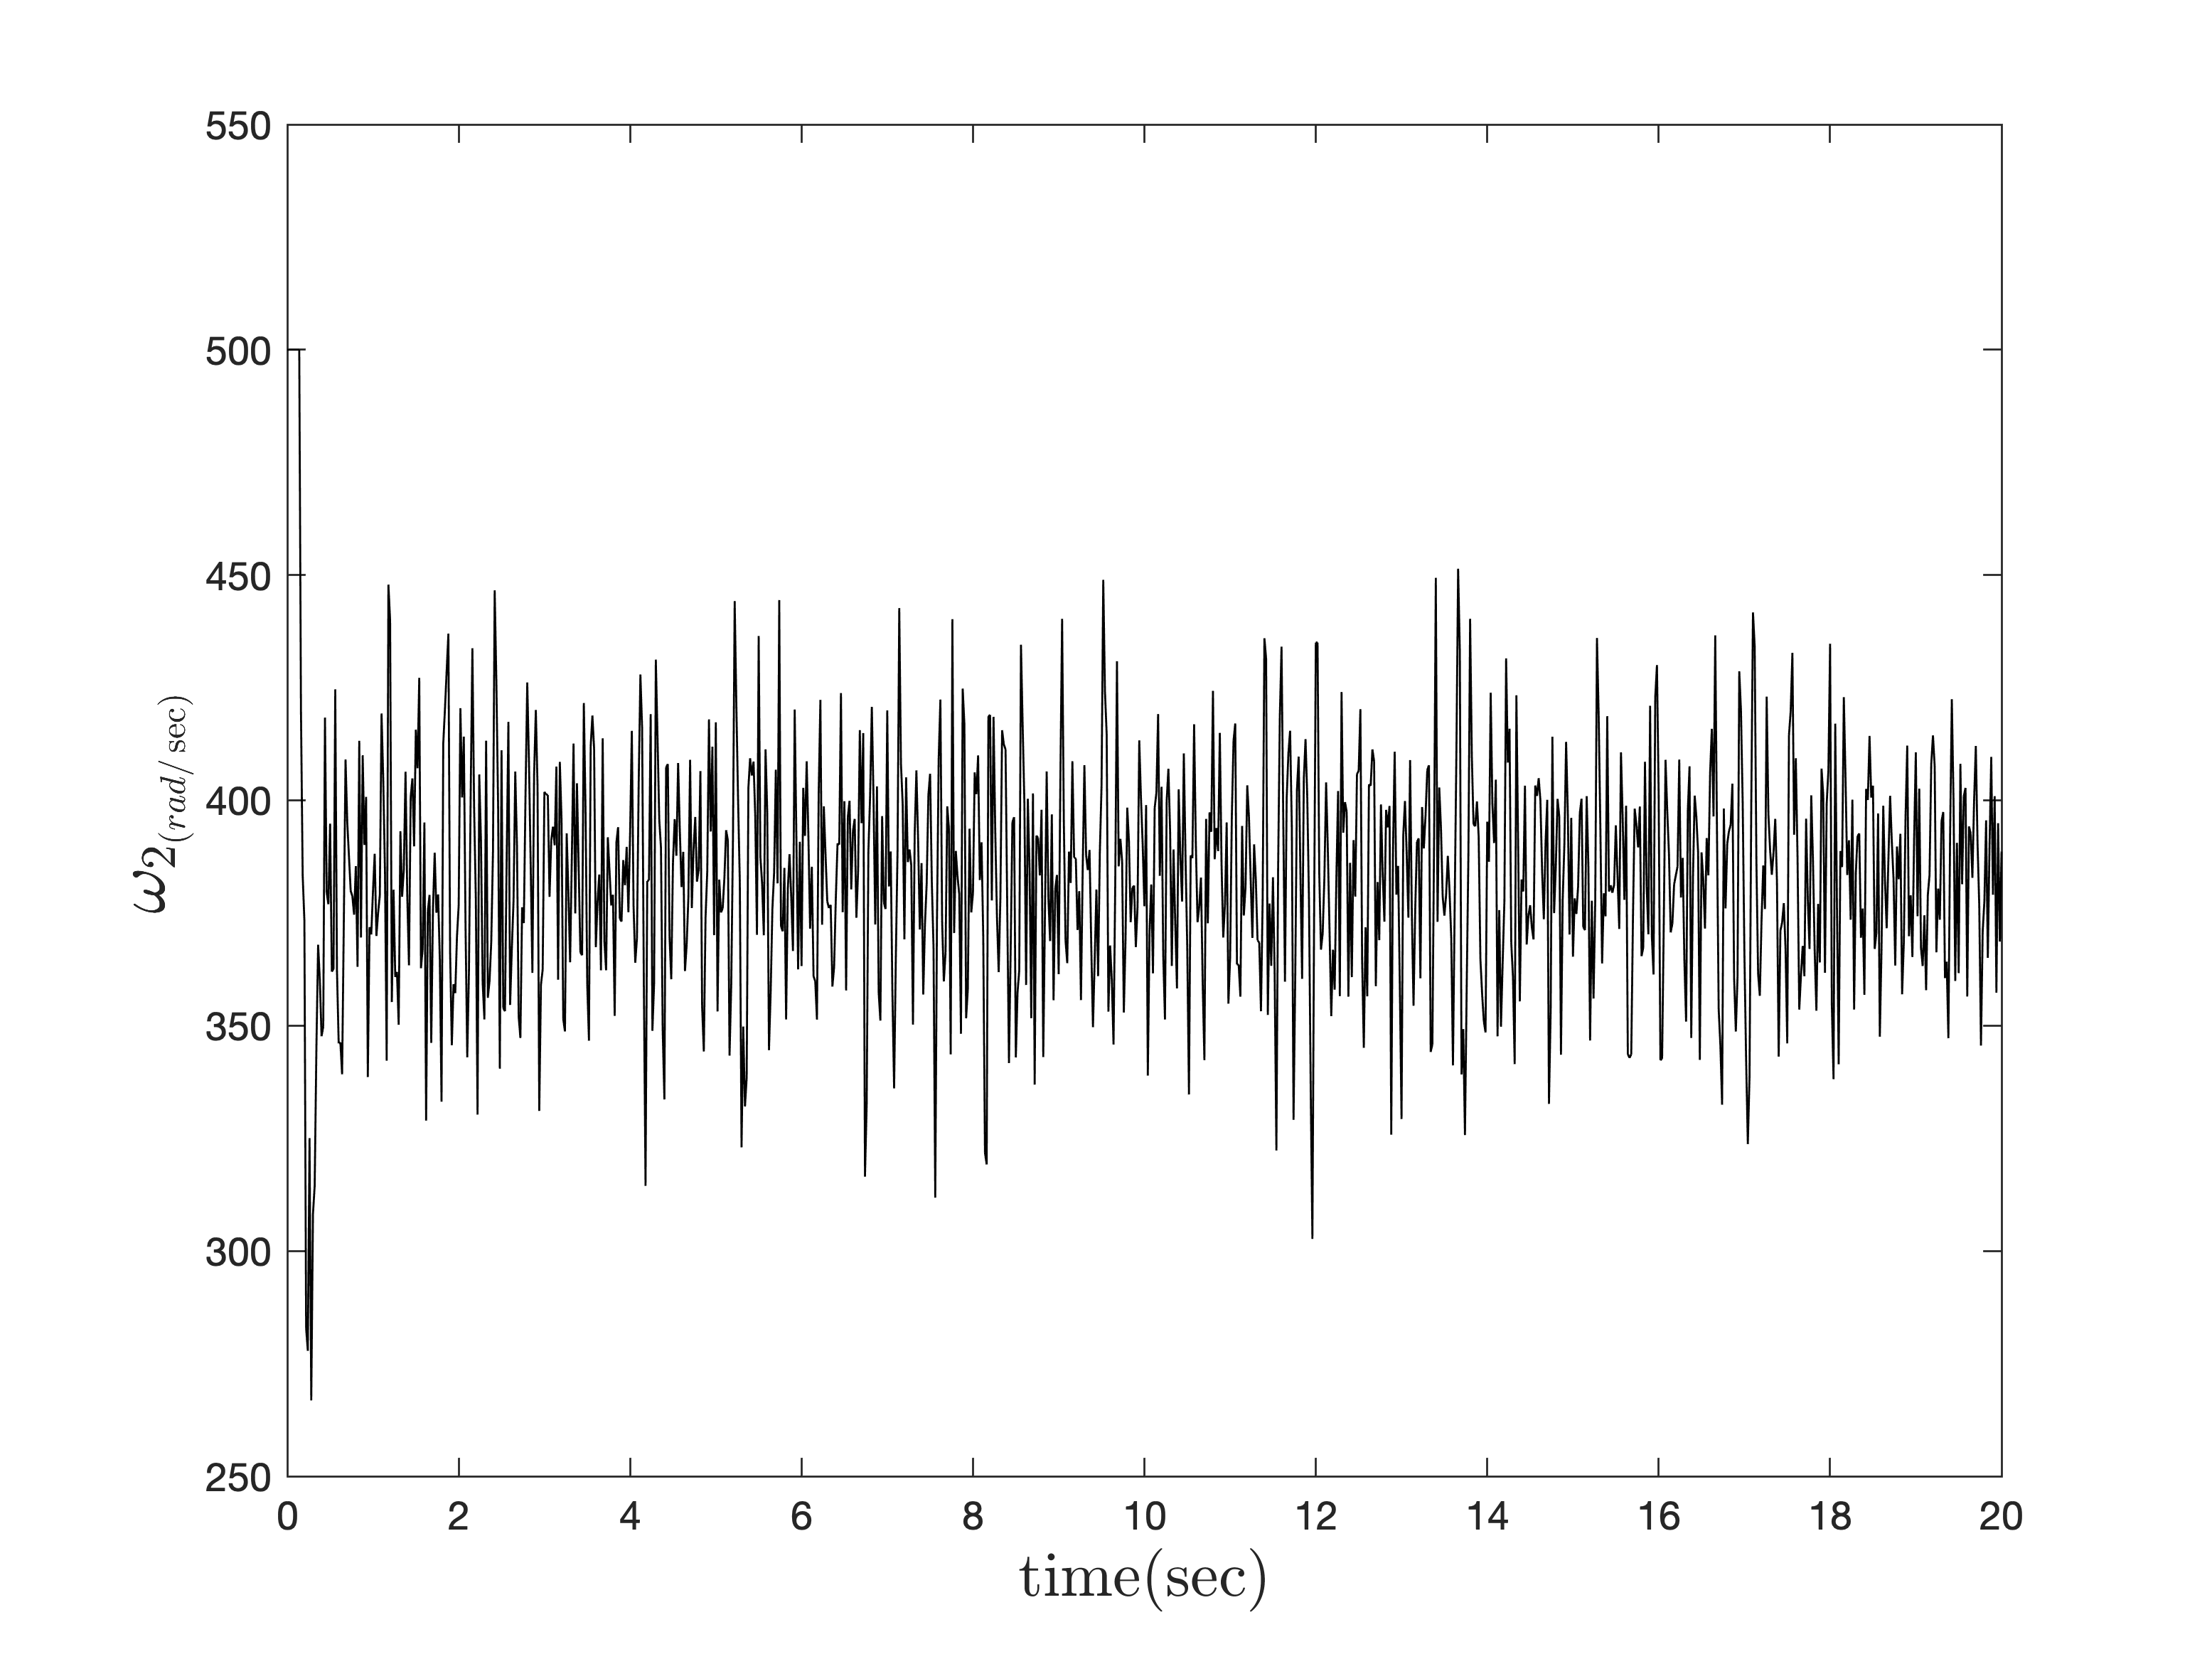
\includegraphics[width=12cm]{../Figures/MIL/LQIDG/Roll_Pitch/lqidg_roll_pitch_Omega_2.png}
	\caption{موتور شماره دو}
\end{subfigure}
	\caption{‫‪فرمان کنترل‌کننده موتور یک و دو در کنترل زاویه رول و پیچ (تعقیب ورودی صفر)}
\end{figure}


\begin{figure}[H]
	\centering
\subfigure[موتور شماره یک]{
		\centering
		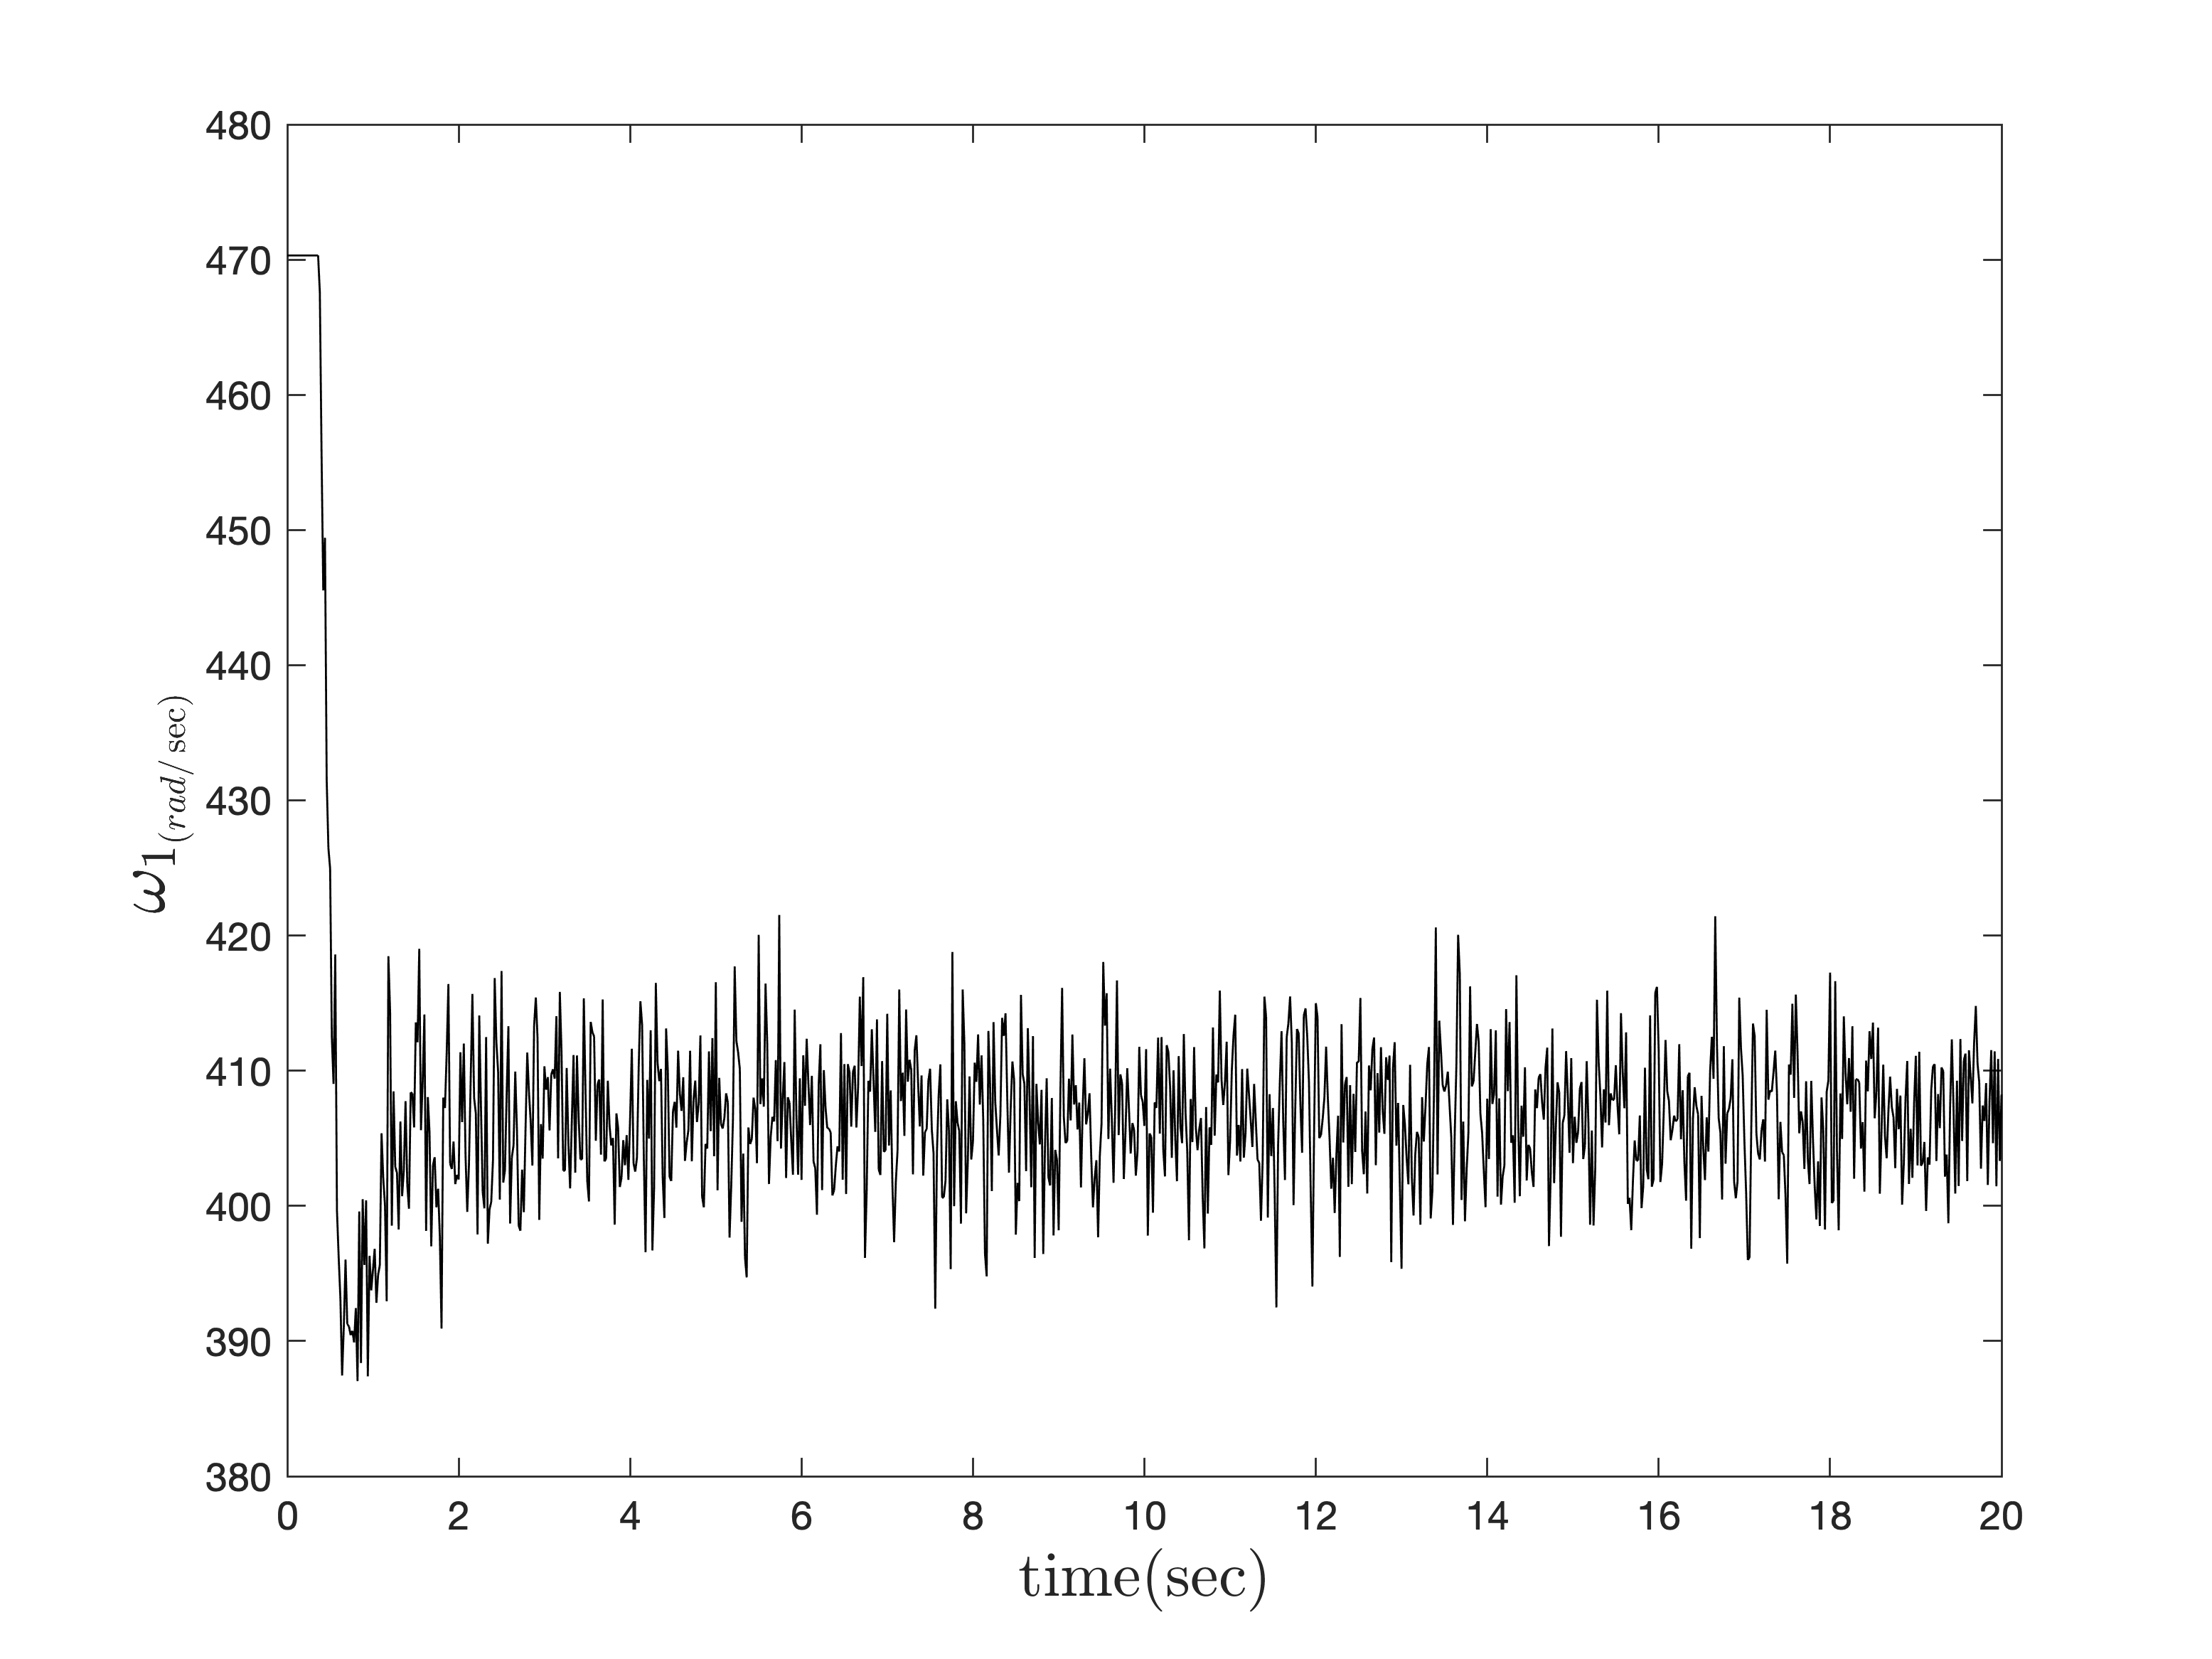
\includegraphics[width=.45\linewidth]{../Figures/MIL/LQIDG/Roll_Pitch/lqidg_roll_pitch_Omega_1.png}
	}
\subfigure[موتور شماره دو]{
	\centering
	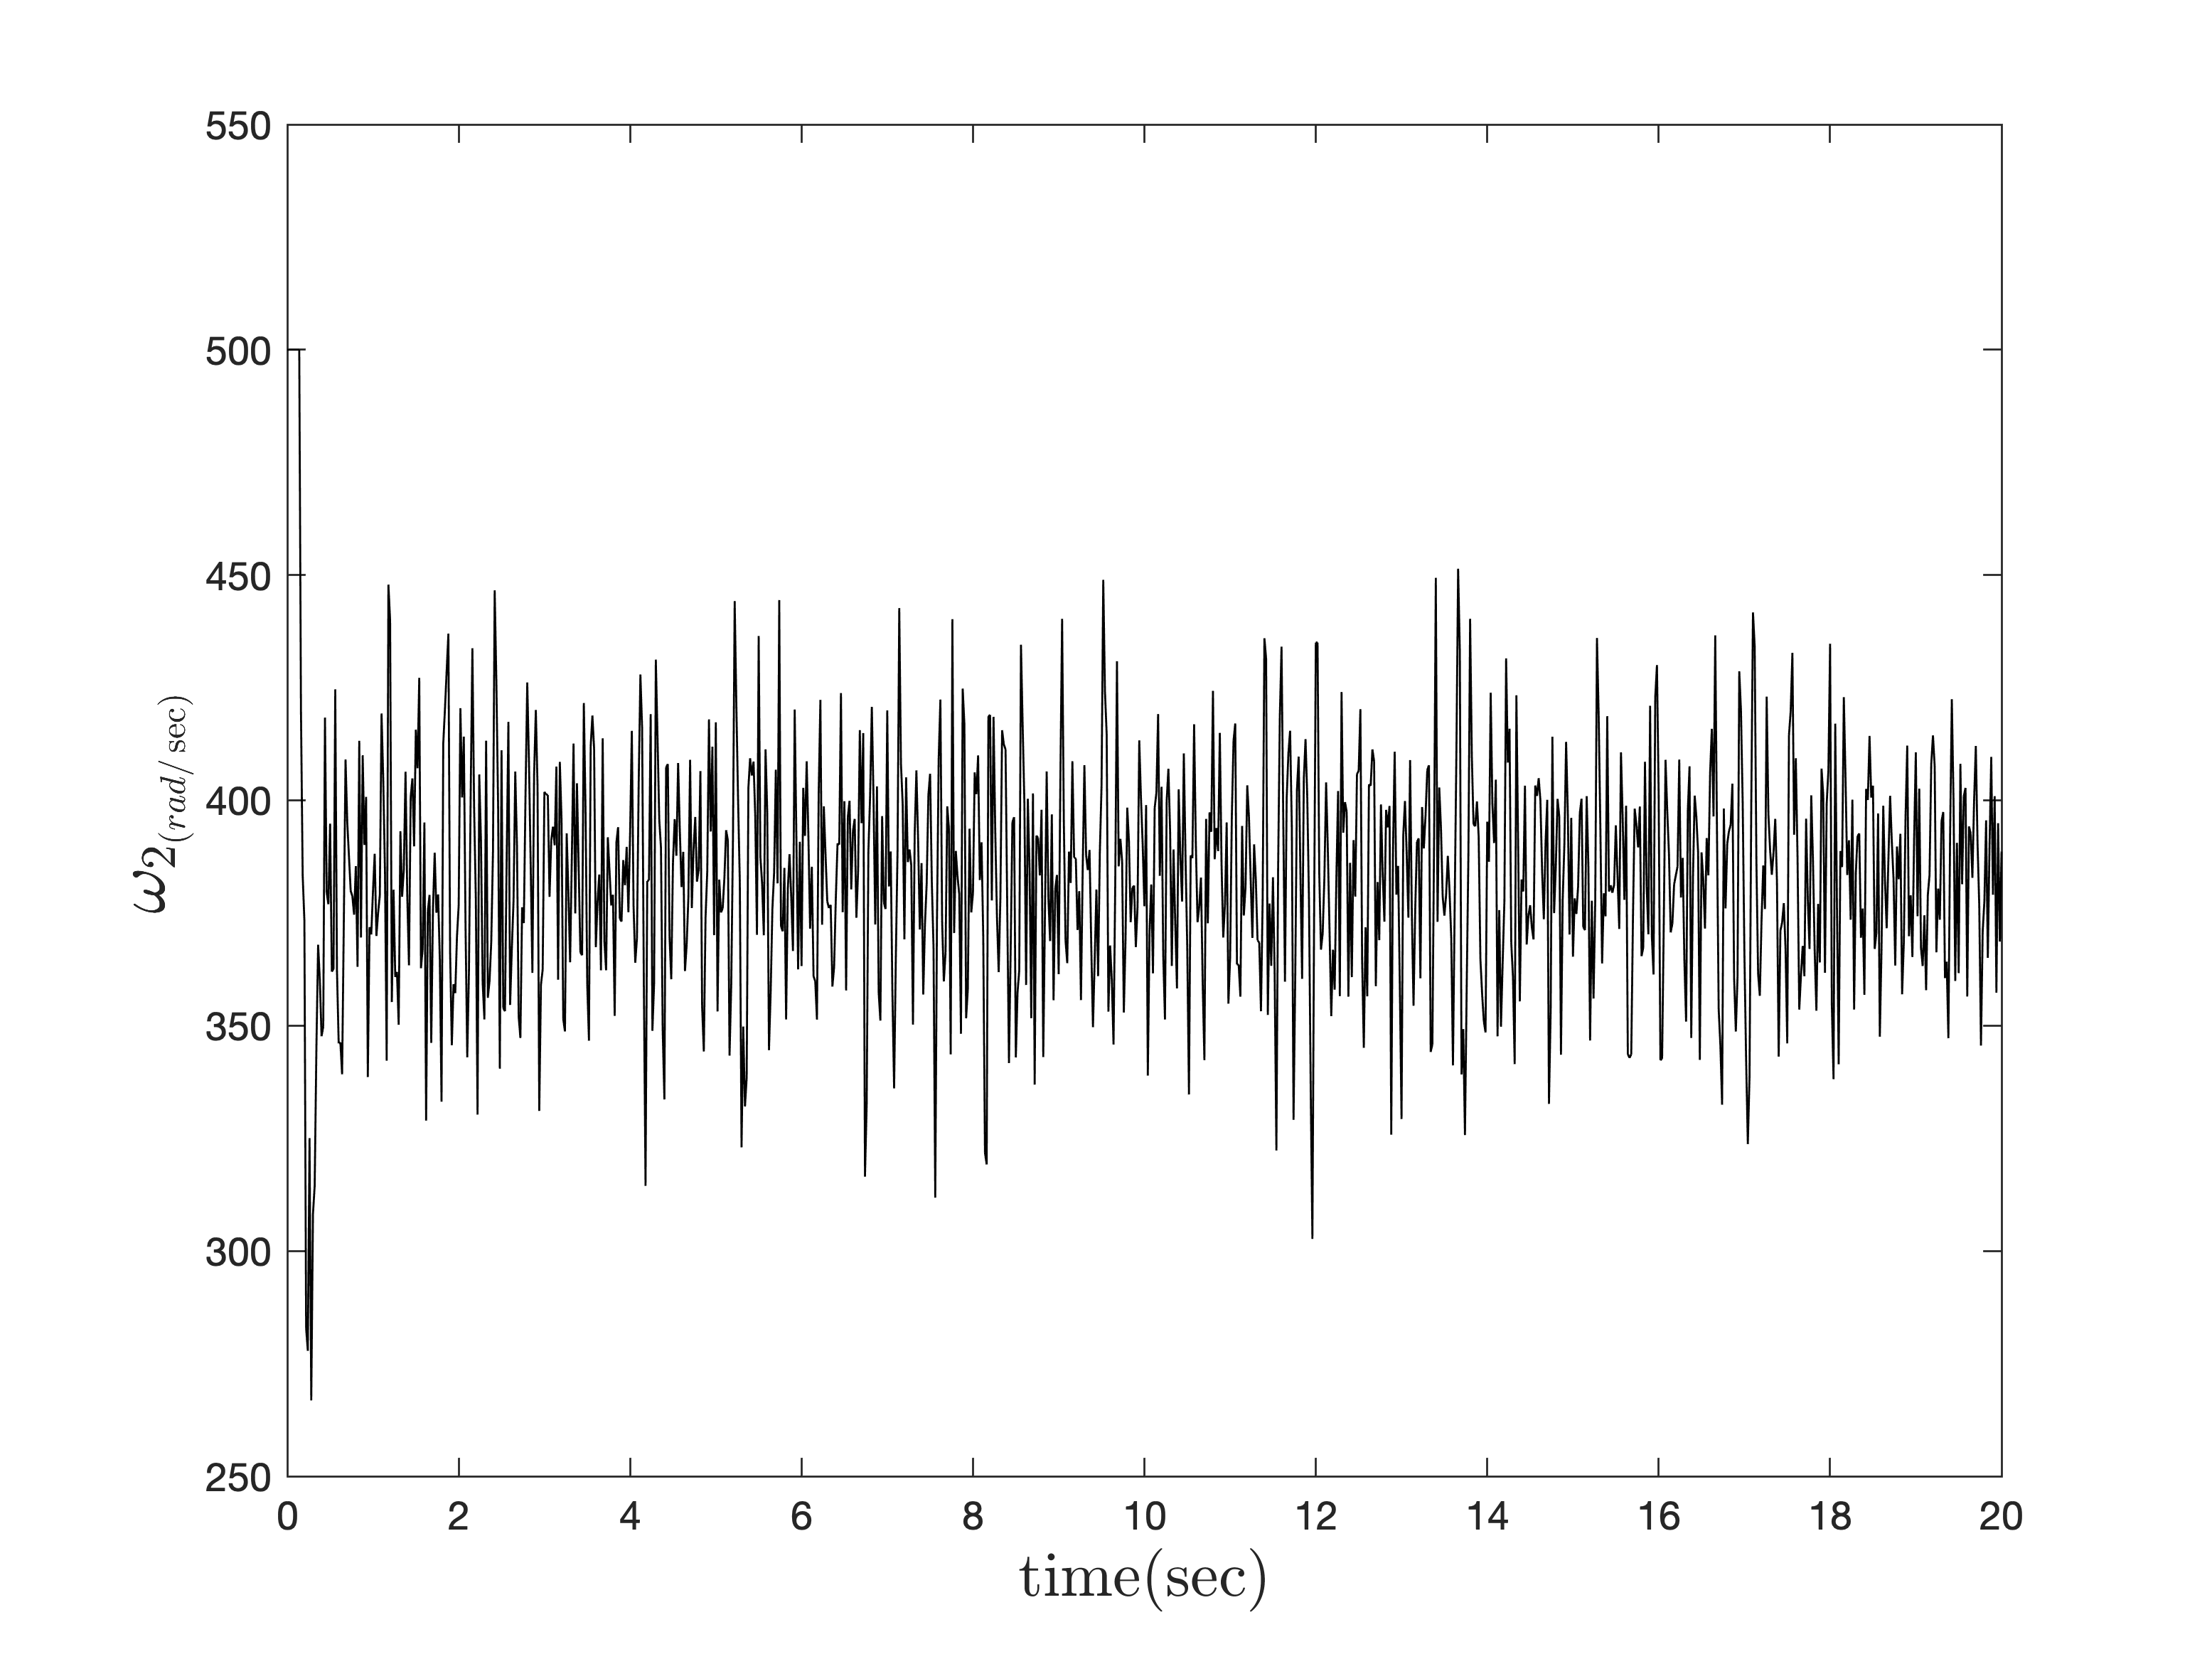
\includegraphics[width=.45\linewidth]{../Figures/MIL/LQIDG/Roll_Pitch/lqidg_roll_pitch_Omega_2.png}
}
\subfigure[موتور شماره سه]{
	\centering
	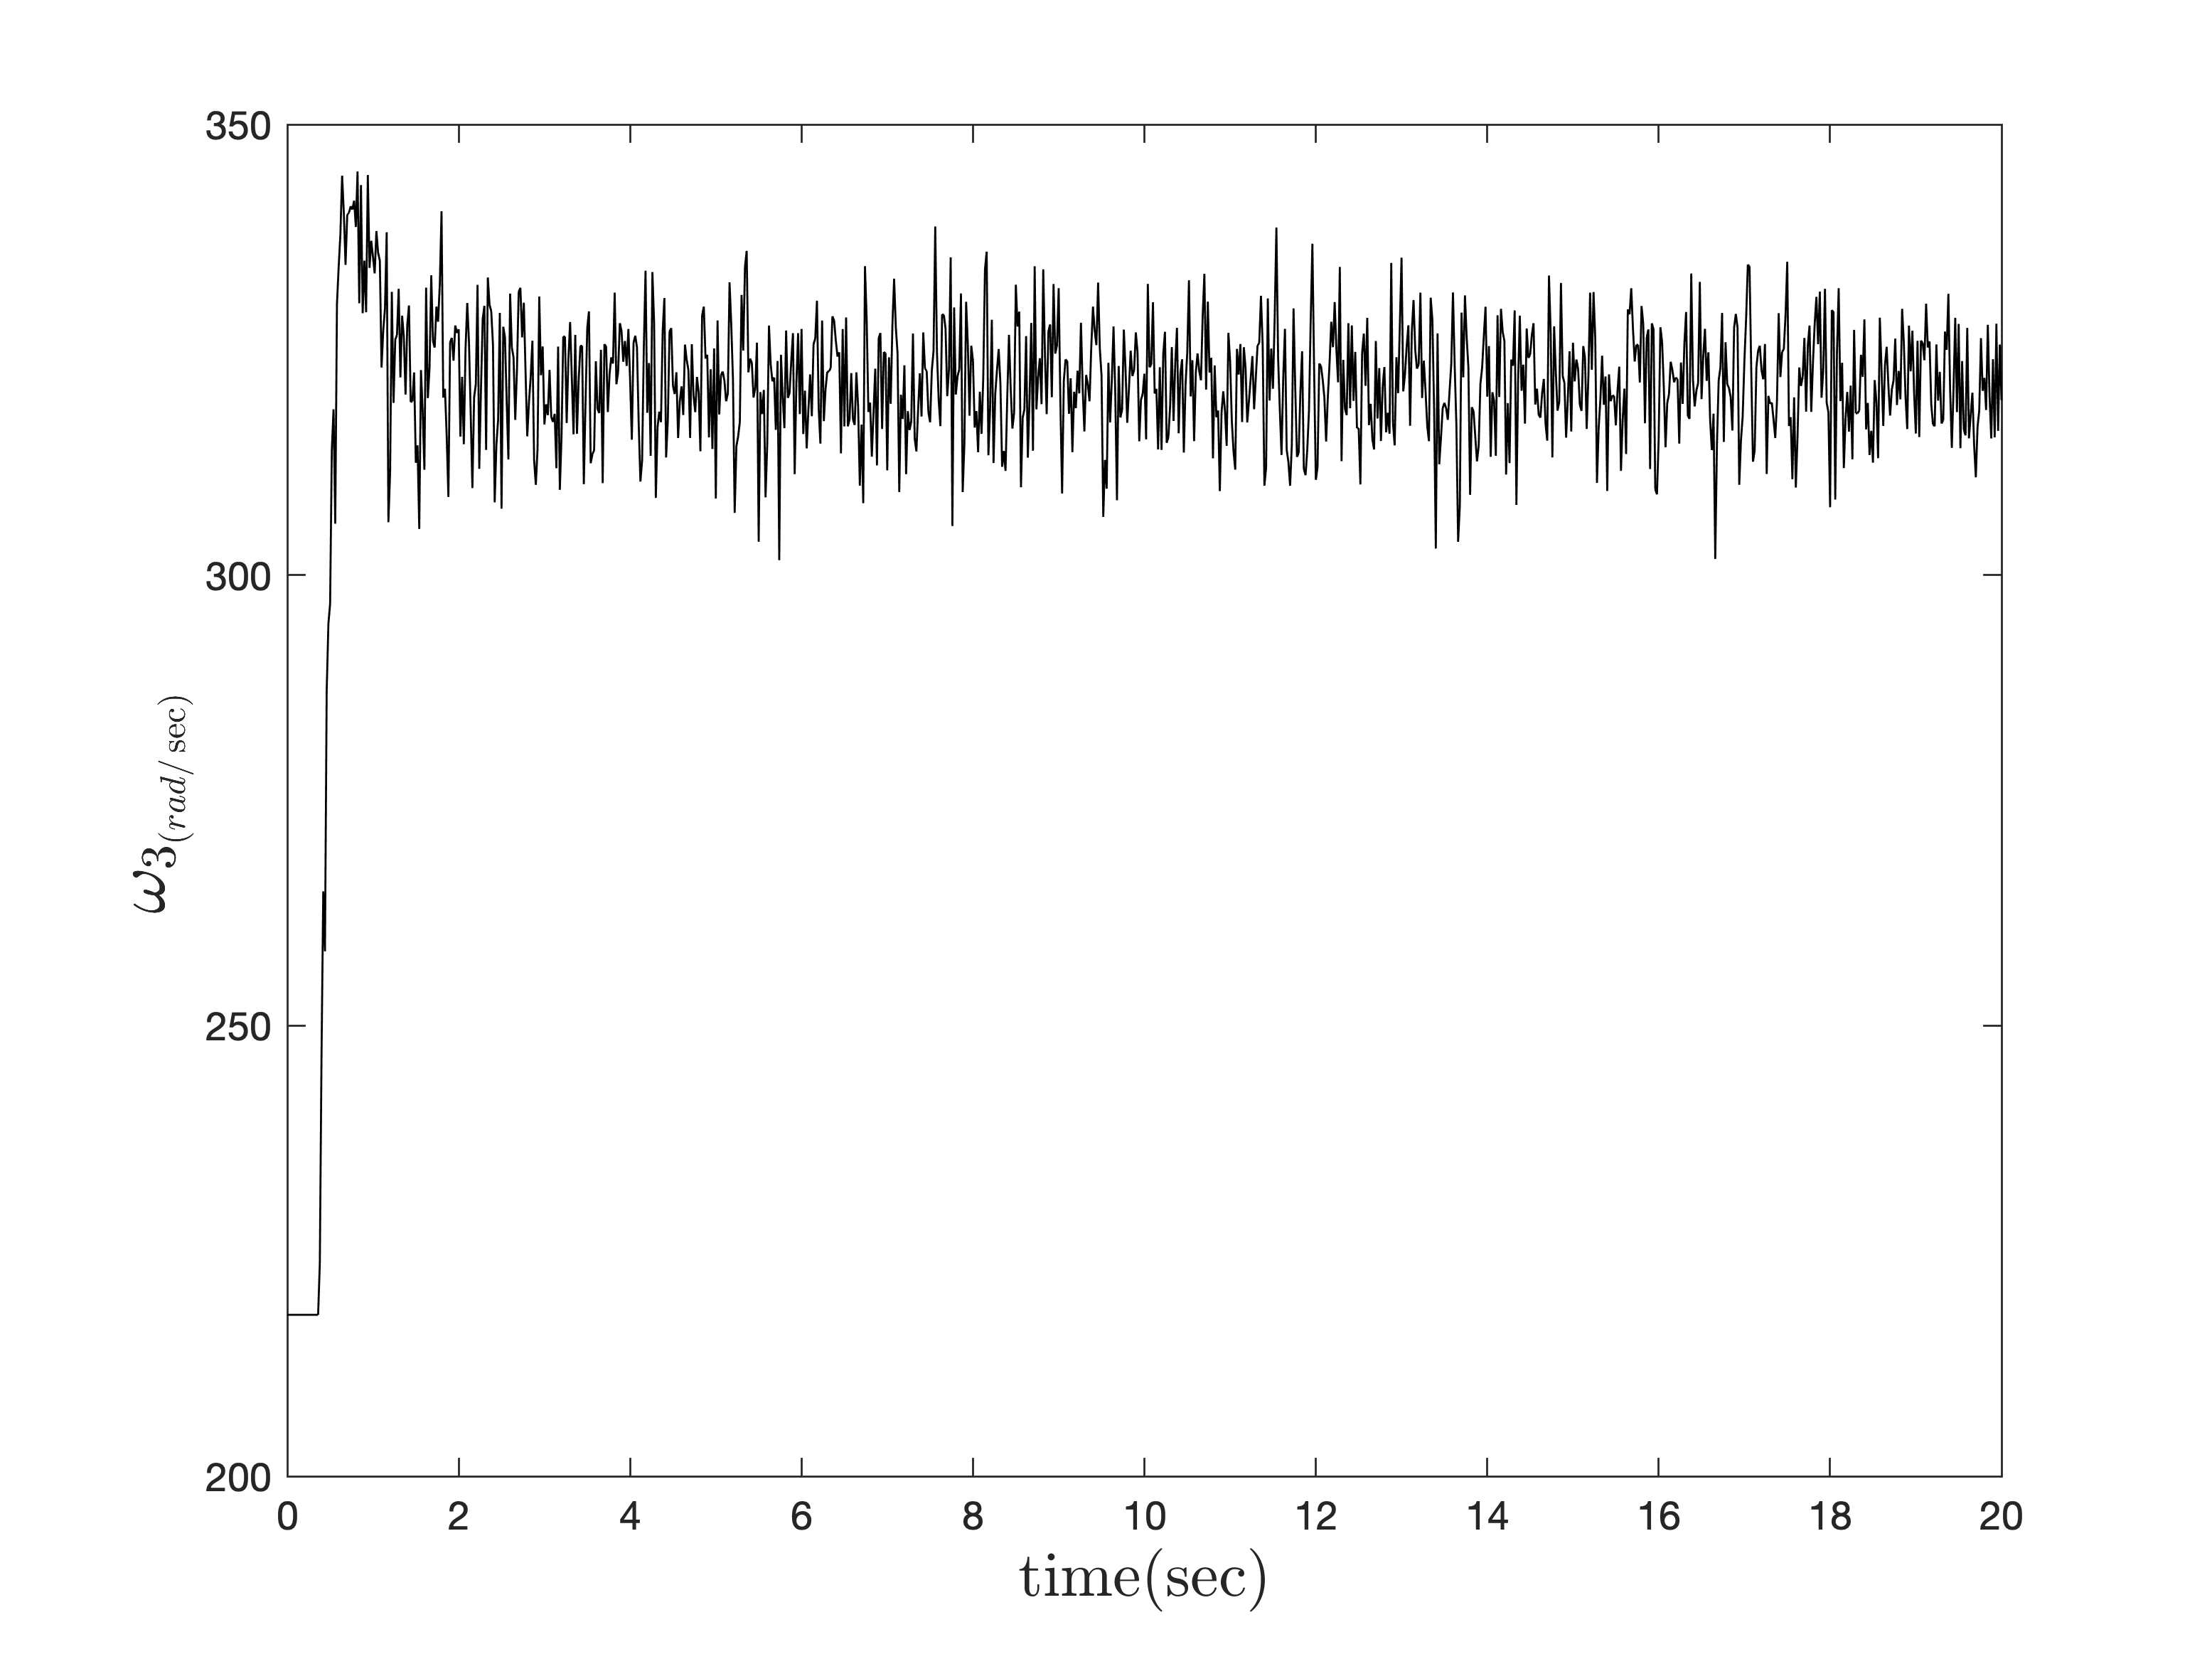
\includegraphics[width=.45\linewidth]{../Figures/MIL/LQIDG/Roll_Pitch/lqidg_roll_pitch_Omega_3.png}
}
\subfigure[موتور شماره چهار]{
	\centering
	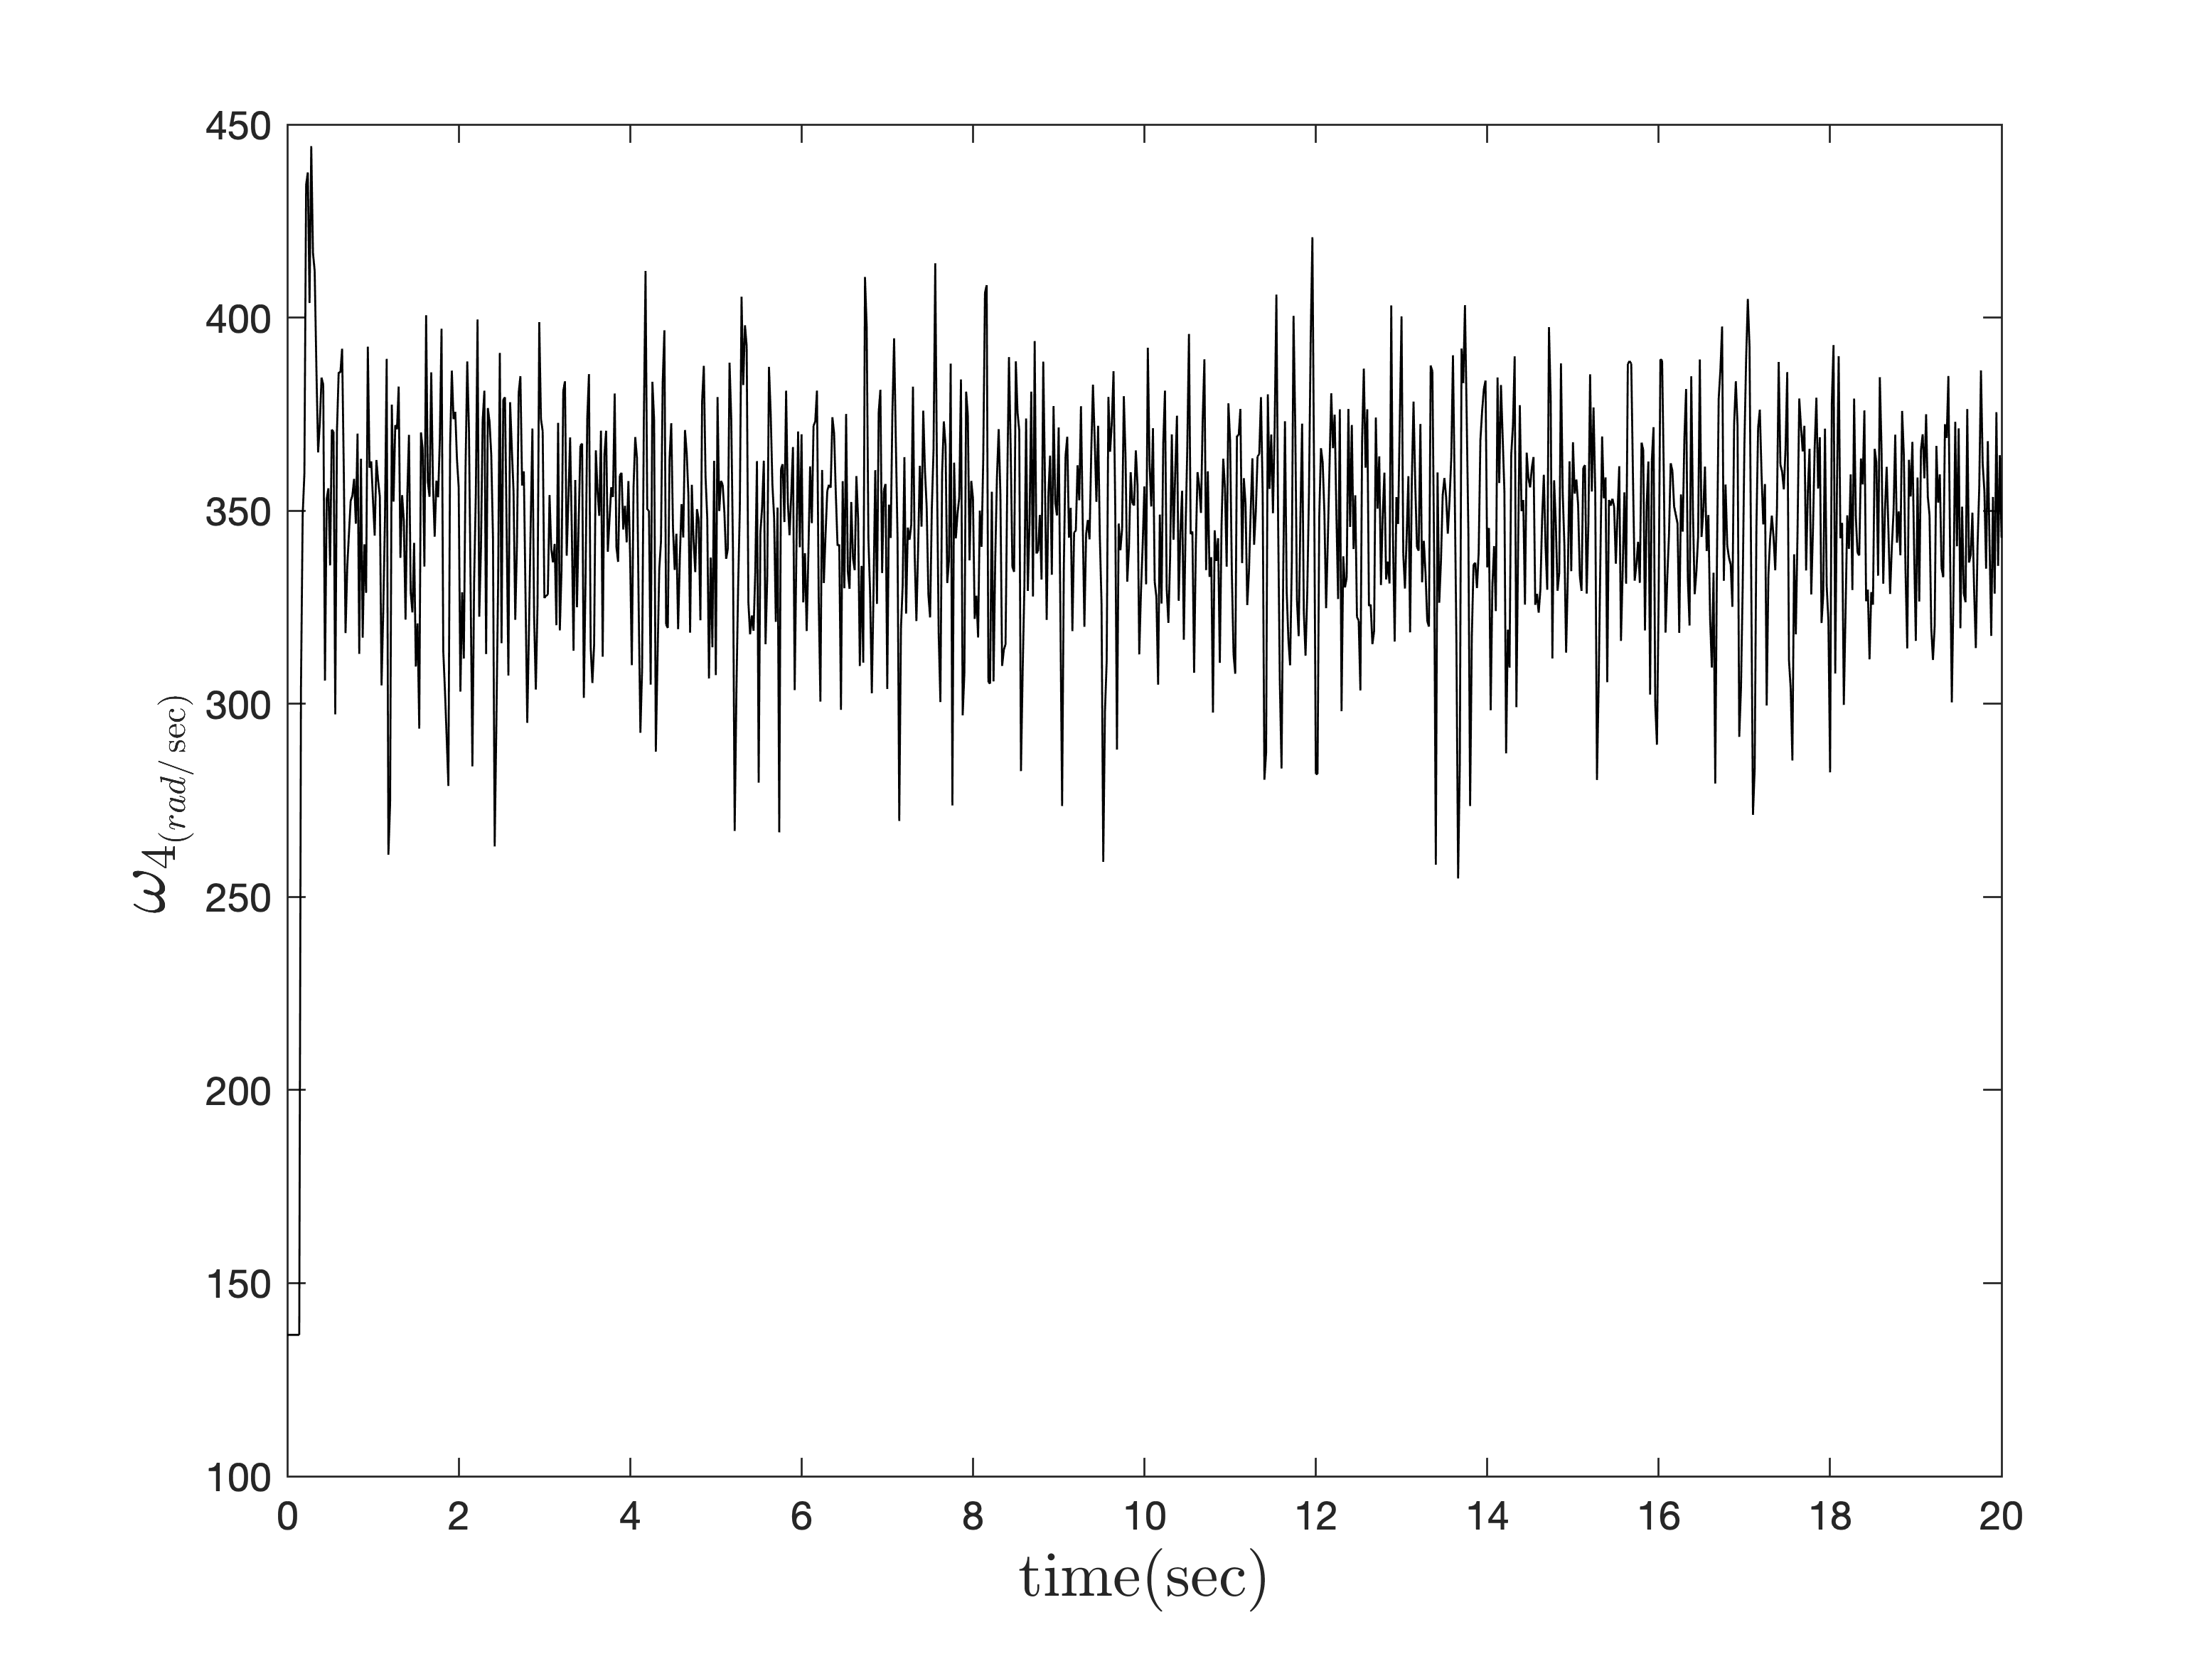
\includegraphics[width=.45\linewidth]{../Figures/MIL/LQIDG/Roll_Pitch/lqidg_roll_pitch_Omega_4.png}
}
	\caption{‫‪فرمان کنترلی موتورها در کنترل زاویه رول و پیچ (تعقیب ورودی صفر)}
\end{figure}


بر اساس خروجی شبیه‌سازی (شکل
\ref{lqidg_roll_fig})
،کانال رول در حضور کنترل‌کننده LQIDG در حدود پنج ثانیه و کانال پیچ در حدود هشت ثانیه به تعادل می‌رسد و خطای ماندگار آن در حدود صفر است.